% ==============================================================================
% RESULTADOS
% ==============================================================================
% Instrucciones de la plantilla:
% - Por cada una de las actividades, describir detalladamente los resultados alcanzados.
% - Incluir capturas de pantalla debidamente tituladas y referenciadas en el texto.
% - REGLA: No se aceptarán solo capturas de pantalla; deben estar explicadas.
% - Analizar ventajas y desventajas de la metodología aplicada.
% ==============================================================================

\section{Resultados}

A continuación se presentan los resultados de cada actividad y de las variaciones. Todas las capturas de OpenGL corresponden al programa compilado en Visual Studio con la configuración \texttt{Debug|x64}.

% ------------------------------------------------------------------------------
\subsection{Resultados de la Actividad 1: hoja en un plano}
En Blender, con el sombreado de material, el plano muestra la hoja recortada y deja ver la cuadrícula del piso alrededor de su contorno (Figura \ref{fig:blender_hoja}). En OpenGL el resultado es el mismo sobre el escenario: la hoja queda tendida en el piso y el fondo se ve a través de las zonas transparentes del plano, sin un recuadro alrededor (Figura \ref{fig:opengl_hoja}). La orilla, suavizada en unos dos píxeles, no muestra escalones al verse en perspectiva.

\begin{figure}[H]
    \centering
    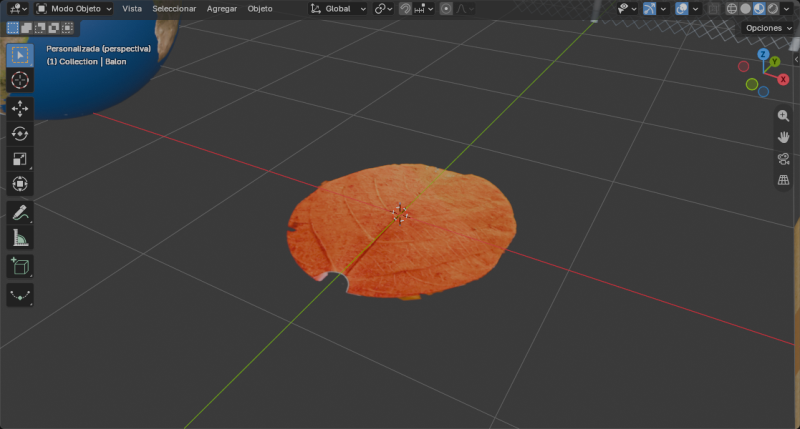
\includegraphics[width=0.6\textwidth]{Imagenes/E1/03_blender_plano_hoja.png}
    \caption{Plano con la textura RGBA de la hoja en la vista de Blender (sombreado de material).}
    \label{fig:blender_hoja}
\end{figure}

\begin{figure}[H]
    \centering
    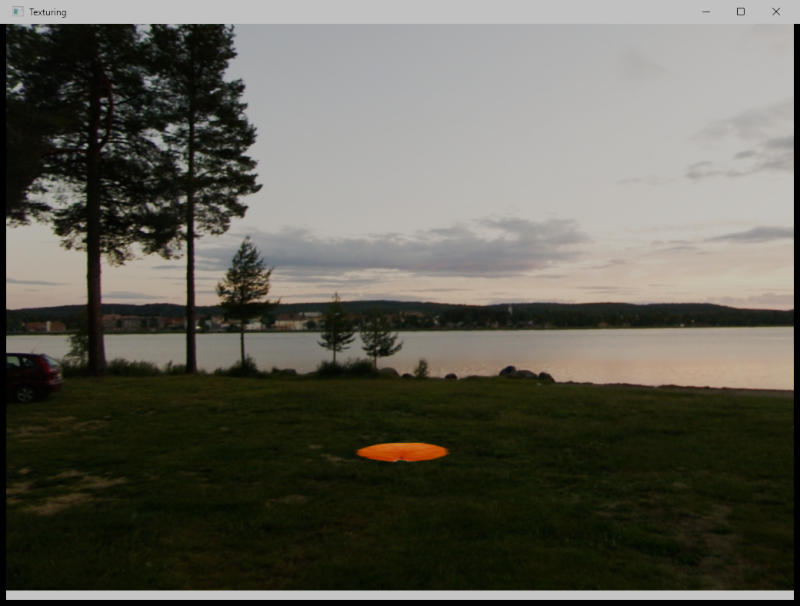
\includegraphics[width=0.6\textwidth]{Imagenes/E1/06_opengl_hoja.png}
    \caption{La hoja en OpenGL sobre el mapa de entorno original: el fondo se ve alrededor de su contorno.}
    \label{fig:opengl_hoja}
\end{figure}

\subsubsection{Análisis de ventajas y desventajas}
\begin{itemize}
    \item \textbf{Ventajas:} Un solo plano de 4 vértices representa un objeto de contorno irregular, que con geometría habría requerido decenas de vértices; y como el alfa se calcula con un guion, el procedimiento se puede repetir con otra fotografía cambiando solo los umbrales.
    \item \textbf{Desventajas:} La hoja es plana y de lado desaparece, y el canal alfa depende de que el objeto tenga un color distinto del fondo: en esta foto hizo falta un límite geométrico adicional para separarlos.
\end{itemize}

% ------------------------------------------------------------------------------
\subsection{Resultados de la Actividad 2: caja de cartón}
La Figura \ref{fig:atlas_caja} muestra el atlas de la caja: la fila inferior contiene el frente, el costado derecho con la cinta que baja y la parte de atrás; la segunda fila, el costado izquierdo, la tapa con la pestaña y la cinta, y el fondo. En Blender (Figura \ref{fig:blender_caja}) se ve que la cinta de la tapa coincide con la que baja por el costado, lo que confirma que la orientación de cada cara en el atlas es la correcta, y que el «arriba» de todos los costados apunta hacia $+Z$.

\begin{figure}[H]
    \centering
    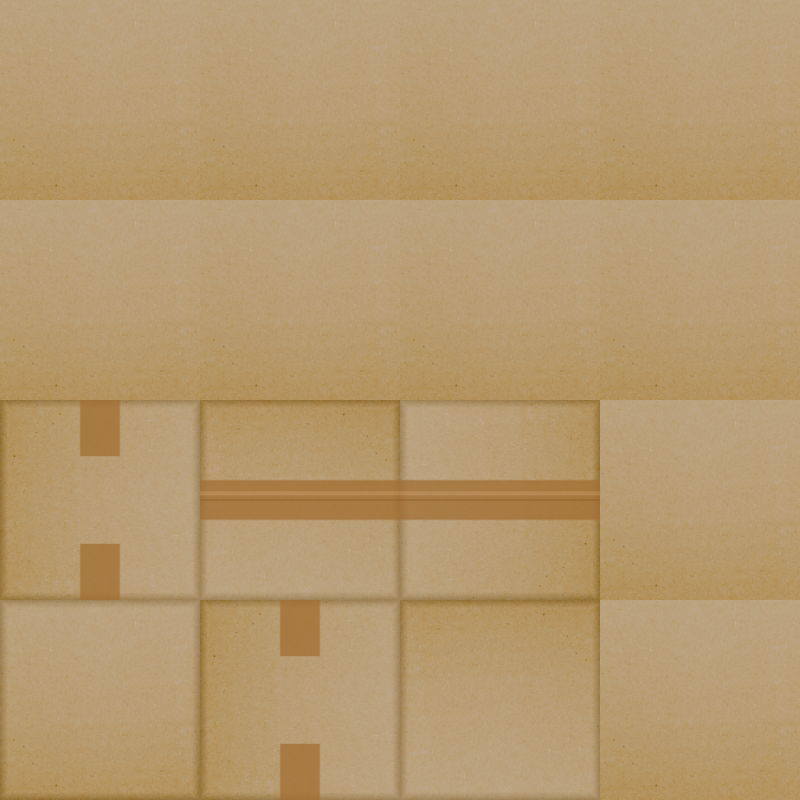
\includegraphics[width=0.45\textwidth]{Imagenes/E2/01_atlas_caja.png}
    \caption{Atlas de la caja ($2048 \times 2048$, cuadrícula de $4 \times 4$ celdas de 512 píxeles, de las que se usan seis).}
    \label{fig:atlas_caja}
\end{figure}

\begin{figure}[H]
    \centering
    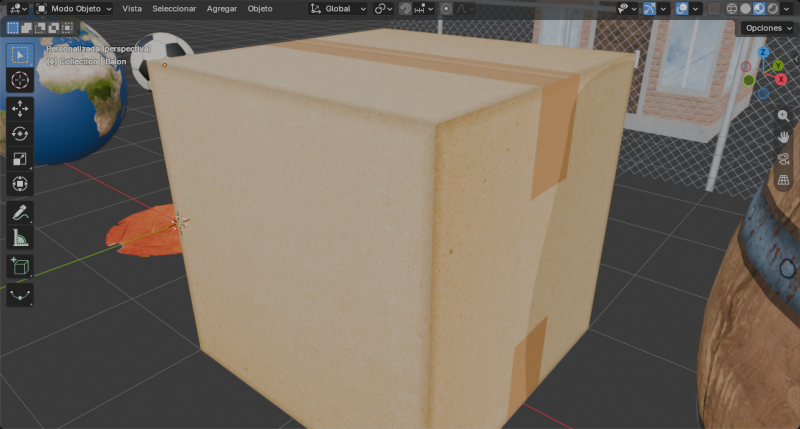
\includegraphics[width=0.6\textwidth]{Imagenes/E2/02_blender_caja.png}
    \caption{La caja de cartón en Blender: la cinta cruza la tapa y continúa por el costado.}
    \label{fig:blender_caja}
\end{figure}

\subsubsection{Análisis de ventajas y desventajas}
\begin{itemize}
    \item \textbf{Ventajas:} Con un atlas, el cubo usa un solo material y una sola textura, que en OpenGL es una sola consulta de imagen; además, cada cara puede llevar un diseño distinto, como la cinta que solo aparece en la tapa, el fondo y dos costados.
    \item \textbf{Desventajas:} Diez de las dieciséis celdas del atlas no se usan, y el margen de 4 píxeles por celda es necesario para que el filtrado no mezcle caras vecinas.
\end{itemize}

% ------------------------------------------------------------------------------
\subsection{Resultados de la Actividad 3: barril}
El atlas del barril (Figura \ref{fig:atlas_barril}) reúne las tres imágenes: las duelas con sus aros y remaches en la mitad superior y las dos tapas en la inferior. En Blender (Figura \ref{fig:blender_barril}) el costado se ve continuo, sin la franja que dejaría la costura, y la forma abombada hace que los aros superior e inferior queden en la parte angosta, como en un barril real. Desde arriba se ve la tapa de tablas oscuras con su borde de acero.

\begin{figure}[H]
    \centering
    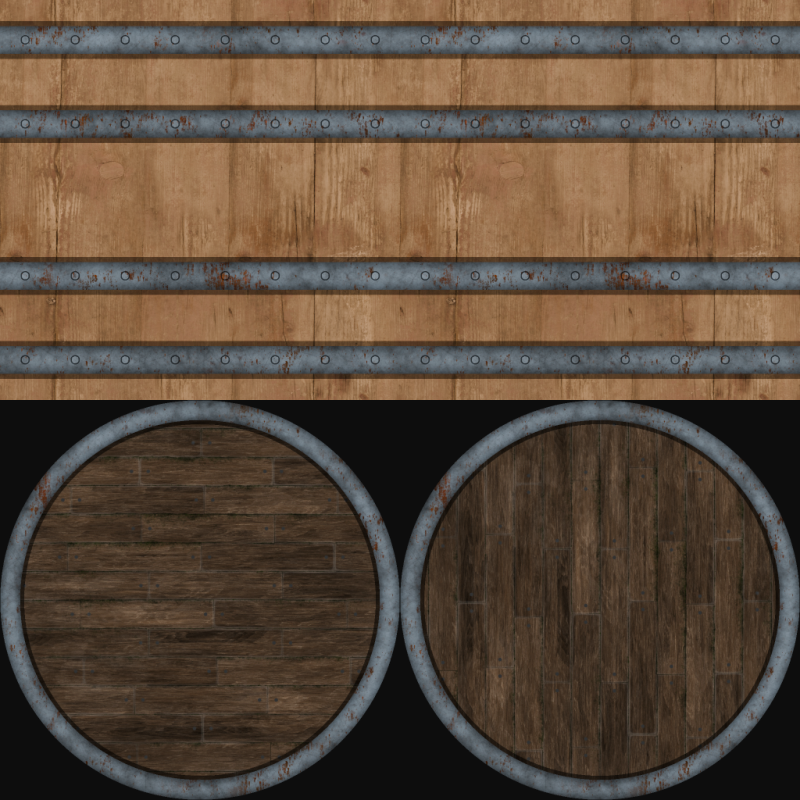
\includegraphics[width=0.45\textwidth]{Imagenes/E3/01_atlas_barril.png}
    \caption{Atlas del barril ($2048 \times 2048$): costado con duelas, aros y remaches arriba; tapa y fondo abajo.}
    \label{fig:atlas_barril}
\end{figure}

\begin{figure}[H]
    \centering
    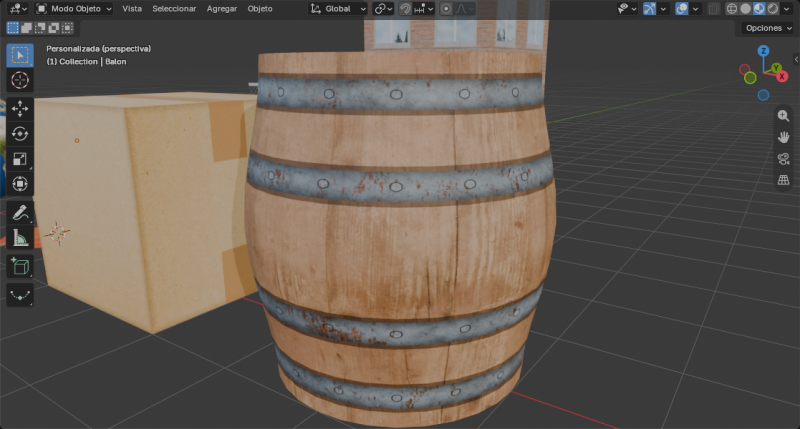
\includegraphics[width=0.48\textwidth]{Imagenes/E3/03_blender_barril.png}
    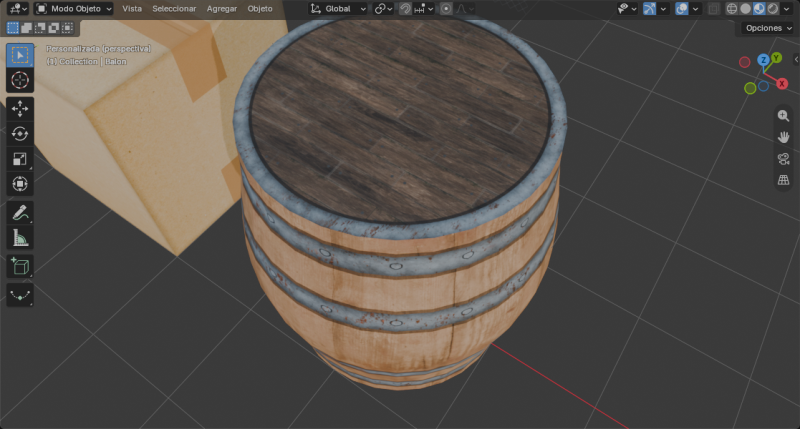
\includegraphics[width=0.48\textwidth]{Imagenes/E3/04_blender_barril_tapa.png}
    \caption{El barril en Blender después de la edición proporcional: costado (izquierda) y vista desde arriba con la tapa (derecha).}
    \label{fig:blender_barril}
\end{figure}

\subsubsection{Análisis de ventajas y desventajas}
\begin{itemize}
    \item \textbf{Ventajas:} La forma se obtuvo escalando un solo anillo, y la edición proporcional repartió el cambio entre los demás de forma suave; como se hizo después de texturizar, las coordenadas UV se conservaron sin trabajo adicional.
    \item \textbf{Desventajas:} Al abombar el costado, la textura se estira un 18\,\% a lo ancho en el centro, porque las coordenadas UV no se recalcularon con la nueva circunferencia; en la madera no se nota, pero en una textura con figuras regulares sí se vería.
\end{itemize}

% ------------------------------------------------------------------------------
\subsection{Resultados de la Actividad 4: planeta}
La Tierra se ve correctamente en Blender y en OpenGL (Figura \ref{fig:planeta}): los continentes conservan su forma y el hielo del Ártico queda arriba, sin pellizcos visibles en los polos gracias a los 32 anillos de la esfera.

\begin{figure}[H]
    \centering
    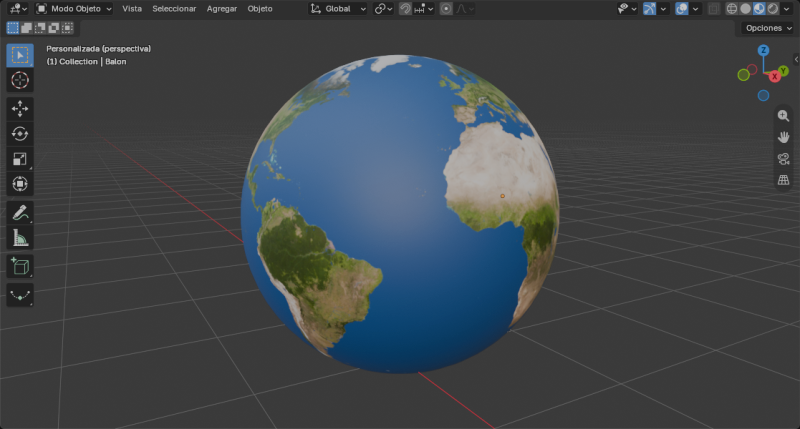
\includegraphics[width=0.48\textwidth]{Imagenes/E4/02_blender_planeta.png}
    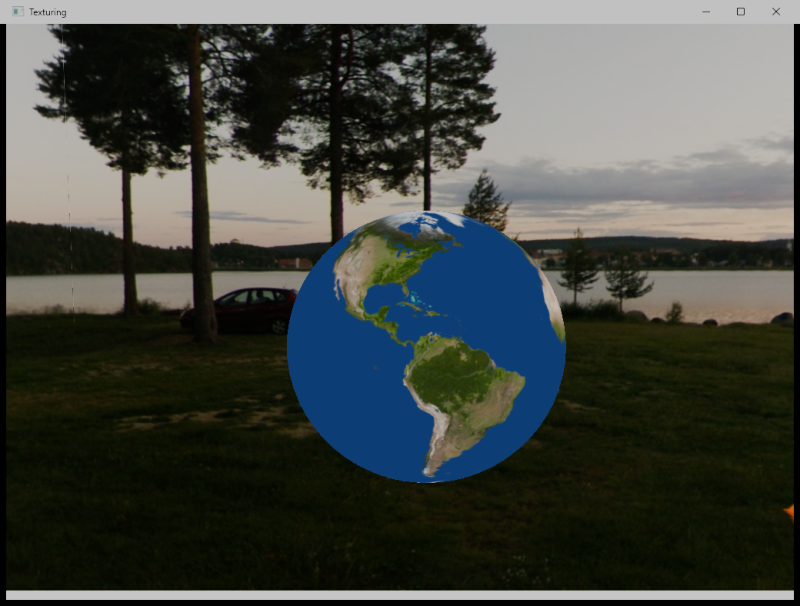
\includegraphics[width=0.48\textwidth]{Imagenes/E4/04_opengl_planeta.png}
    \caption{El planeta en Blender (izquierda) y en OpenGL (derecha).}
    \label{fig:planeta}
\end{figure}

\subsubsection{Análisis de ventajas y desventajas}
\begin{itemize}
    \item \textbf{Ventajas:} La esfera UV y la proyección equirrectangular son compatibles de origen, así que cualquier mapa de planeta se aplica sin desplegar nada.
    \item \textbf{Desventajas:} La proyección equirrectangular desperdicia resolución cerca de los polos, donde toda una fila de la imagen se concentra en un círculo pequeño, y los triángulos de los polos convergen en un solo vértice.
\end{itemize}

% ------------------------------------------------------------------------------
\subsection{Resultados de la Actividad 5: escena exportada a OpenGL}
Las cuatro figuras del manual se exportan juntas y aparecen en OpenGL en la misma disposición que en Blender (Figura \ref{fig:escena_actividades}): el planeta, la hoja, la caja y el barril, de izquierda a derecha. El archivo \texttt{escena\_p6.fbx} con las ocho figuras pesa 209 KB, y las texturas que se copian a \texttt{bin/models} suman unos 16 MB.

\begin{figure}[H]
    \centering
    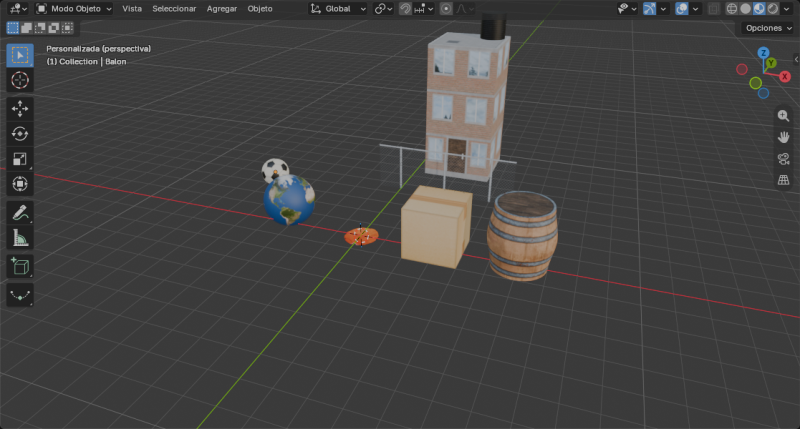
\includegraphics[width=0.48\textwidth]{Imagenes/E5/01_blender_escena_actividades.png}
    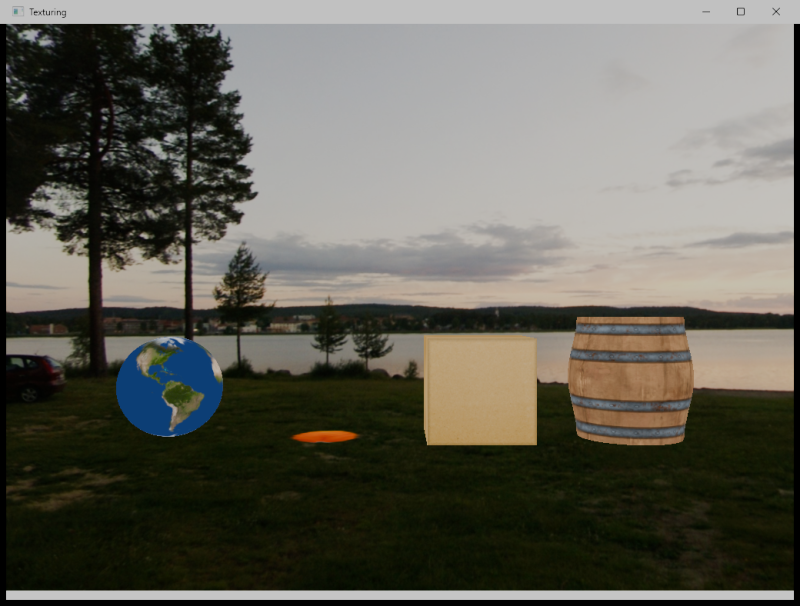
\includegraphics[width=0.48\textwidth]{Imagenes/E3/06_opengl_barril_forma.png}
    \caption{Las cuatro figuras de las actividades en Blender (izquierda) y en OpenGL (derecha).}
    \label{fig:escena_actividades}
\end{figure}

\subsubsection{Análisis de ventajas y desventajas}
\begin{itemize}
    \item \textbf{Ventajas:} Exportar copias con la transformación aplicada resuelve la limitación del cargador sin modificar el \texttt{.blend}, y las correcciones a \texttt{model.h} y al \textit{shader} quedaron como cambios pequeños y explicados.
    \item \textbf{Desventajas:} Al ir todo en un solo modelo, las figuras comparten la matriz de modelo y no se pueden mover por separado desde el programa.
\end{itemize}

% ------------------------------------------------------------------------------
\subsection{Resultados de la Actividad 6: nuevo mapa de entorno}
La Figura \ref{fig:cambio_fondo} compara la misma escena con el mapa de entorno original del laboratorio y con el cubemap \textit{Footballfield}. El cambio no requirió tocar el modelo del cubo ni sus coordenadas de textura, solo las seis imágenes y una ruta en el código. Con la cancha de fondo, el pasto continúa visualmente el piso sobre el que están las figuras y la escena gana coherencia con el balón y la reja.

\begin{figure}[H]
    \centering
    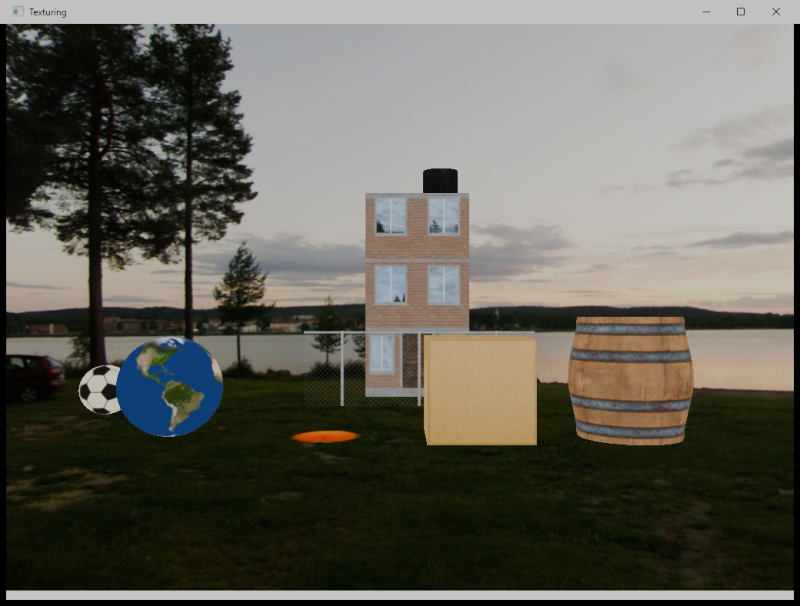
\includegraphics[width=0.48\textwidth]{Imagenes/E6/02_opengl_fondo_original.png}
    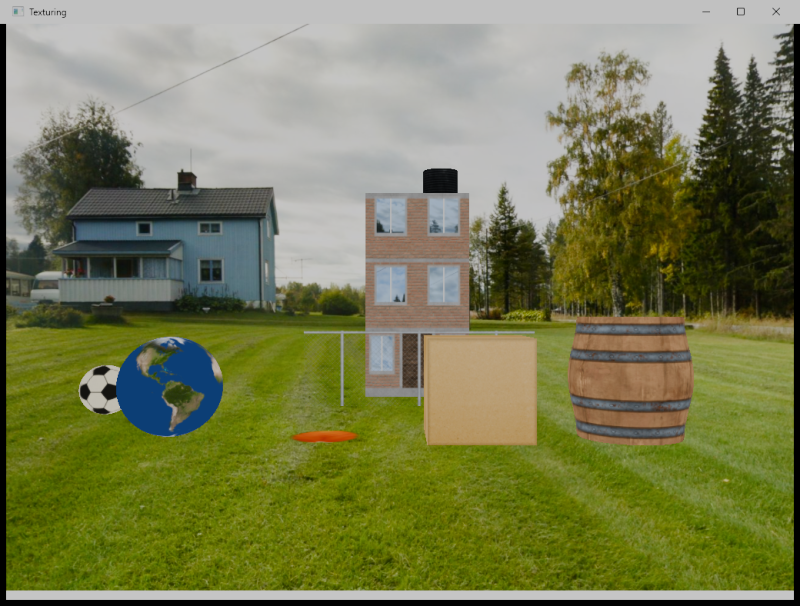
\includegraphics[width=0.48\textwidth]{Imagenes/E6/03_opengl_fondo_cancha.png}
    \caption{La escena con el mapa de entorno original (izquierda) y con el cubemap \textit{Footballfield} de Humus (derecha).}
    \label{fig:cambio_fondo}
\end{figure}

\subsubsection{Análisis de ventajas y desventajas}
\begin{itemize}
    \item \textbf{Ventajas:} Seis imágenes de $2048 \times 2048$ dan un fondo fotográfico completo a cualquier dirección de la cámara con solo doce triángulos.
    \item \textbf{Desventajas:} El fondo no tiene paralaje: al mover la cámara, los árboles y la casa del fondo se desplazan junto con ella, y las figuras no proyectan sombra sobre el pasto de la imagen.
\end{itemize}

% ------------------------------------------------------------------------------
\subsection{Resultados de las variaciones}
La Figura \ref{fig:texturas_variaciones} reúne las cuatro texturas generadas. En la reja, el magenta es la parte transparente y solo quedan opacos los rombos, el poste y el tubo, que suman el 16\,\% de la imagen. En el atlas del edificio se distinguen las cuatro fachadas con la puerta en la planta baja de la primera, y en la textura equirrectangular del balón, los 12 pentágonos y 20 hexágonos deformados por la proyección.

\begin{figure}[H]
    \centering
    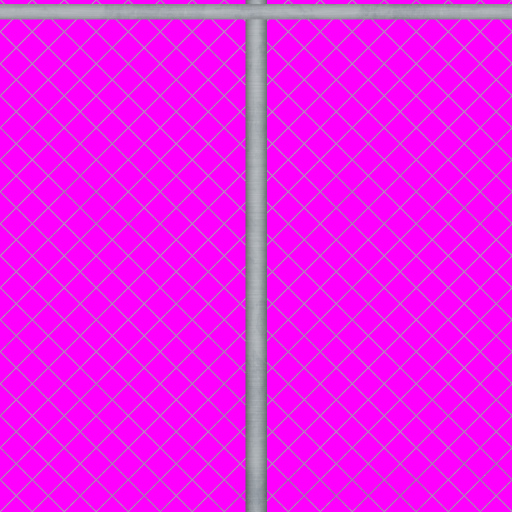
\includegraphics[width=0.24\textwidth]{Imagenes/V/01_reja_rgba_magenta.png}
    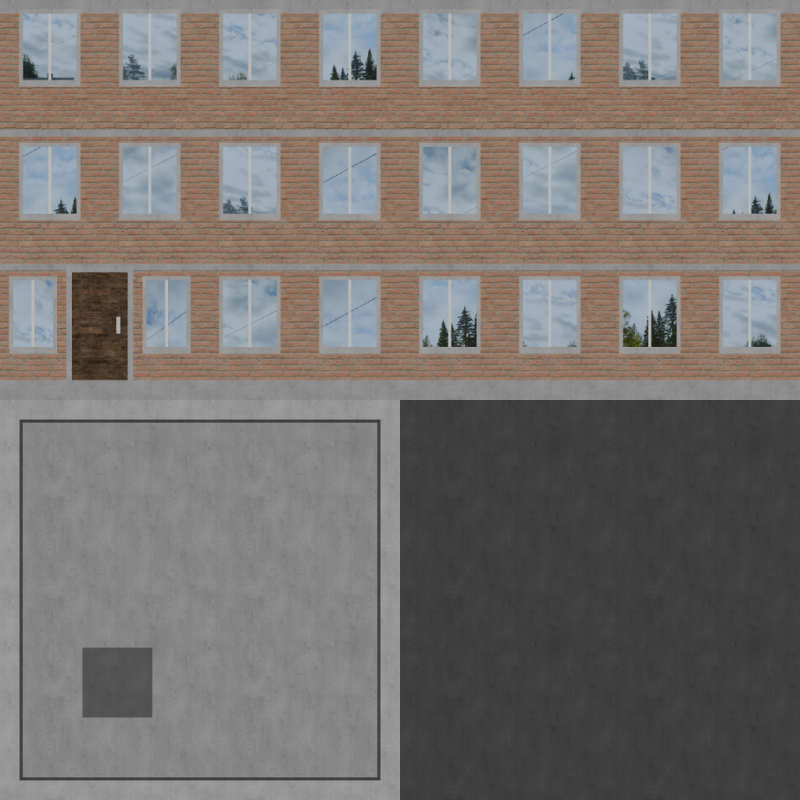
\includegraphics[width=0.24\textwidth]{Imagenes/V/02_atlas_edificio.png}
    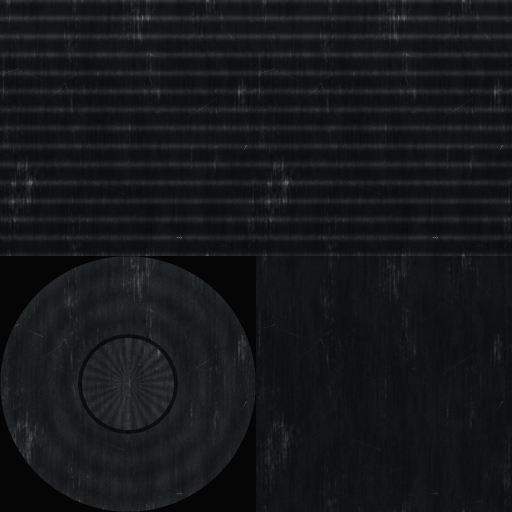
\includegraphics[width=0.24\textwidth]{Imagenes/V/03_atlas_tinaco.png}\\[0.2cm]
    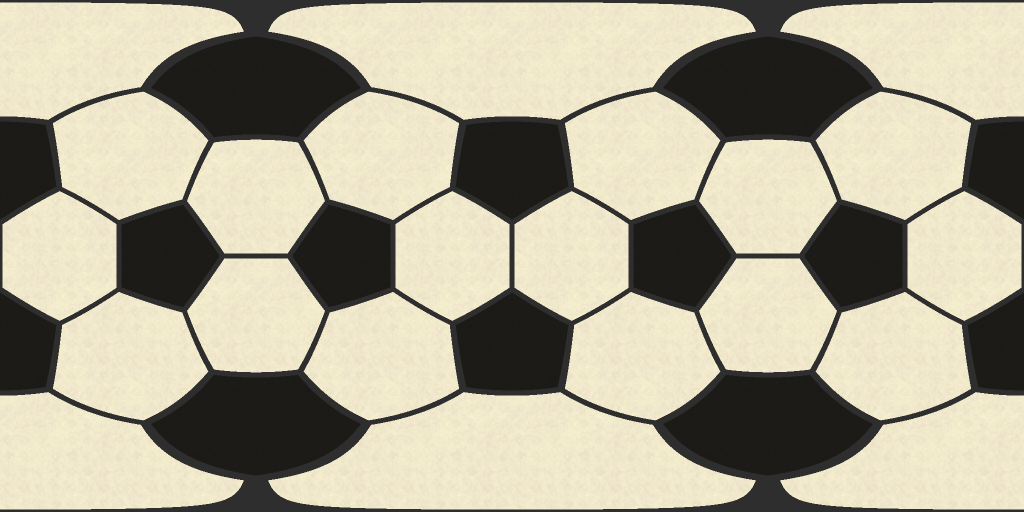
\includegraphics[width=0.6\textwidth]{Imagenes/V/04_textura_balon.png}
    \caption{Texturas de las variaciones: reja sobre magenta, atlas del edificio y atlas del tinaco (arriba), y textura equirrectangular del balón (abajo).}
    \label{fig:texturas_variaciones}
\end{figure}

En Blender (Figura \ref{fig:variaciones_blender}) el edificio muestra sus ventanas con el reflejo del cielo, la puerta, las losas de cada piso y el tinaco sobre la azotea; detrás de la reja se ve la fachada a través de los rombos, y el balón tiene el patrón completo de pentágonos y hexágonos.

\begin{figure}[H]
    \centering
    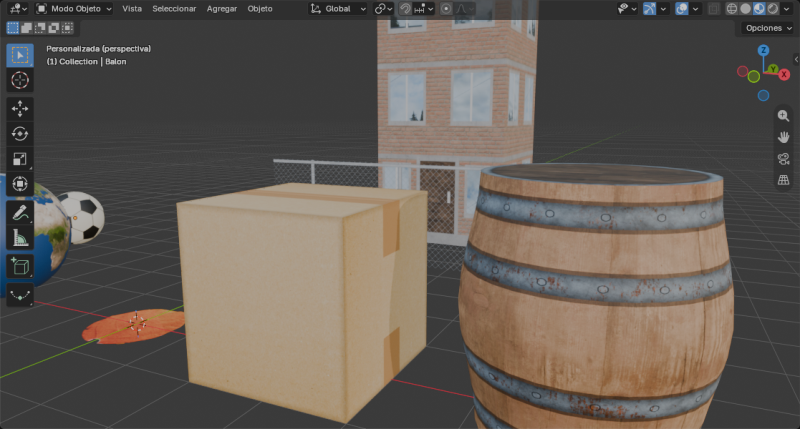
\includegraphics[width=0.32\textwidth]{Imagenes/V/05_blender_reja.png}
    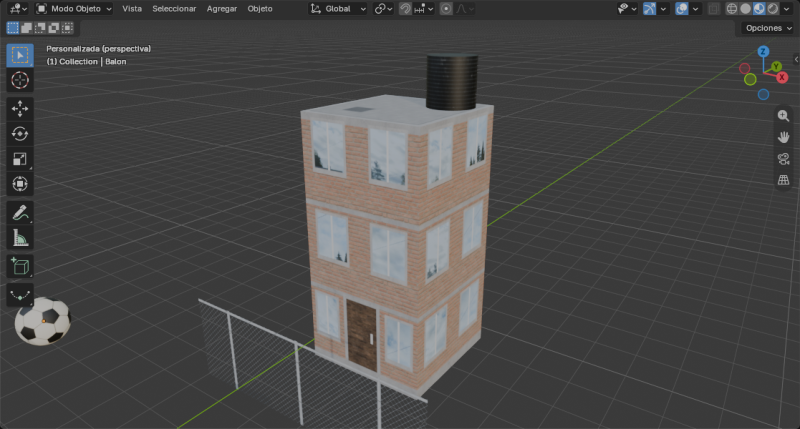
\includegraphics[width=0.32\textwidth]{Imagenes/V/06_blender_edificio_tinaco.png}
    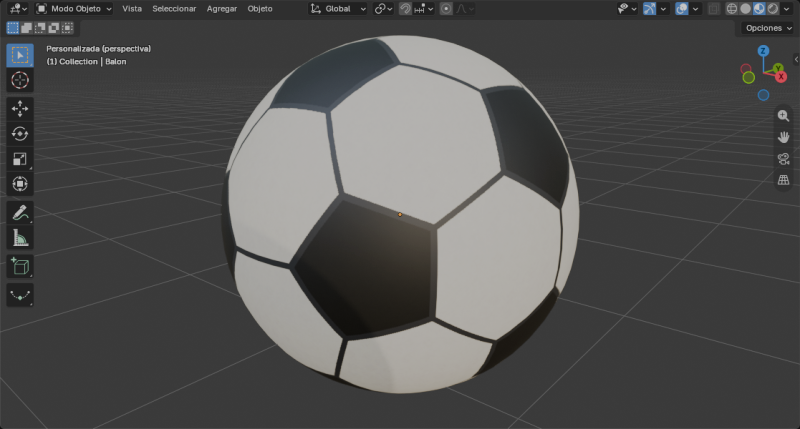
\includegraphics[width=0.32\textwidth]{Imagenes/V/07_blender_balon.png}
    \caption{Variaciones en Blender: reja con el edificio detrás (izquierda), edificio con tinaco (centro) y balón de fútbol (derecha).}
    \label{fig:variaciones_blender}
\end{figure}

Finalmente, la Figura \ref{fig:escena_completa} muestra la escena completa. En OpenGL, la reja es transparente sin que la fachada que está detrás desaparezca, el tinaco queda sobre la azotea y el balón junto al planeta.

\begin{figure}[H]
    \centering
    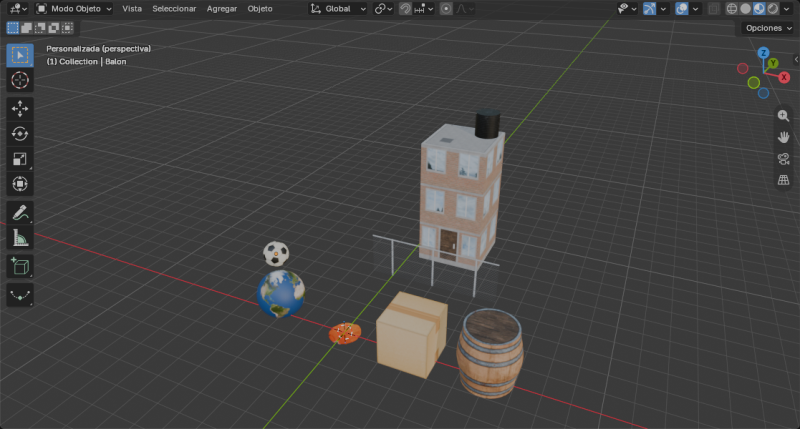
\includegraphics[width=0.48\textwidth]{Imagenes/V/08_blender_escena_completa.png}
    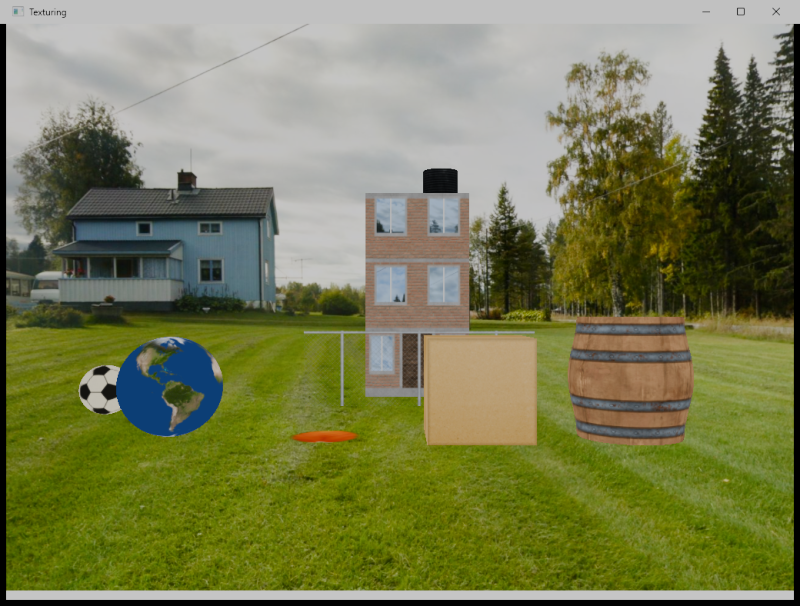
\includegraphics[width=0.48\textwidth]{Imagenes/E6/03_opengl_fondo_cancha.png}
    \caption{Las ocho figuras en Blender (izquierda) y en OpenGL con el nuevo mapa de entorno (derecha).}
    \label{fig:escena_completa}
\end{figure}

\subsubsection{Análisis de ventajas y desventajas}
\begin{itemize}
    \item \textbf{Ventajas:} Las variaciones reutilizaron las mismas técnicas de las actividades con otros parámetros, y las texturas calculadas (la malla de la reja y el balón) no dependen de encontrar una imagen adecuada en internet y se pueden generar a cualquier resolución.
    \item \textbf{Desventajas:} Las ventanas del edificio son solo textura y reflejan un cielo fijo que no cambia con el punto de vista; y el tinaco, al estar en el mismo modelo que el edificio, no se puede mover por separado en OpenGL.
\end{itemize}
